% -*- mode: latex; mode: auto-fill; coding: utf-8; -*-

\documentclass[a4paper,english]{report} 

\usepackage{fullpage}
\usepackage{subfig}
\usepackage[usenames,dvipsnames]{color}

\def\documentstate{final} % Lav om til FINAL når vi er done!
\usepackage[utf8]{inputenc}
\usepackage[\documentstate]{fixme} % kræver at folk er smarte nok til at installere FiXme
\usepackage[T1]{fontenc}
\usepackage{babel}
%\usepackage{lmodern} % vector font, ikke bitmap!!
% ^- kun interessant med latex, pdflatex er vector i forvejen
\usepackage{graphicx}
\graphicspath{{graphics/}}
\DeclareGraphicsExtensions{.pdf,.jpeg,.jpg,.png}
\usepackage{tikz}

\usepackage{wrapfig}
\usepackage[plainpages=false]{hyperref}
\hypersetup{pdfborder=0 0 0} % Go away you ugly boxes!

\usepackage{verbatim}
\usepackage{tikz}
%\usepackage{subfig}
%\usepackage{slashbox}
%\usepackage{color}
\usepackage{listings}
\usepackage{listing}
\usepackage[round]{natbib}
%\renewcommand{\danishhyphenmins}{22} % fuck lorte orddeling!
\usepackage[\documentstate]{ifdraft}
\ifdraft{
  \usepackage{draftwatermark}
  \SetWatermarkScale{4.0}
}{}

%% default lst options

%% Special environments

\newenvironment{shcode}%
{\verbatim}{\endverbatim}

% use a TT font with bold 
\renewcommand{\ttdefault}{pcr}

\lstset{basicstyle=\ttfamily \footnotesize}
\lstset{keywordstyle=\textbf}
\lstset{commentstyle=\normalfont \textit}
\lstset{stringstyle=\bfseries}
\lstset{showstringspaces=false}

\lstset{frameround=tttt}
\lstset{frame=tLBr}

\lstnewenvironment{pythoncode}{\lstset{language=Python}}{}
\lstnewenvironment{cppcode}{\lstset{language=C++}}{}
% \lstnewenvironment{shcode}{\lstset{language=sh}}{}

%% Some commands
\newcommand{\todo}[1]{\textcolor{red}{#1}\fixme{#1}}

\newcommand{\class}[1]{\texttt{#1}}
\newcommand{\method}[1]{\texttt{#1}}
\newcommand{\file}[1]{\texttt{#1}}
\newcommand{\code}[1]{\texttt{#1}}

%%% Local Variables: 
%%% mode: latex
%%% TeX-master: "master"
%%% TeX-PDF-mode: t
%%% End: 


\newcommand{\reffig}[1]{figure \ref{#1}}
\newcommand{\reflst}[1]{listing \ref{#1}}

\newcommand{\citebook}[2]{[\citealp[#1]{#2}]}
\newcommand{\citeabook}[1]{[\citealp{#1}]}

\citestyle{chicago} % Chicago Manual of Style citations
\bibliographystyle{is-alpha} % is- shows ISBN in references

%\title{Rendering natural looking outdoor environments}
%\author{
%  Asger Dam Hoedt \\ asgerhoedt@gmail.com \\ 20051770  \and 
%  Christian P. V. Christoffersen \\ cpvc@cs.au.dk \\ 20050879
%}




\begin{document}

\begin{titlepage}
\pagenumbering{alph}

\thispagestyle{empty}
\centering
{ \baselineskip=24pt
    \vspace*{80pt}
    {\LARGE Rendering natural looking outdoor environments}\\
    Couse: Introduction to Computer Graphics, spring 2010
    \vspace*{20pt}
    \\
    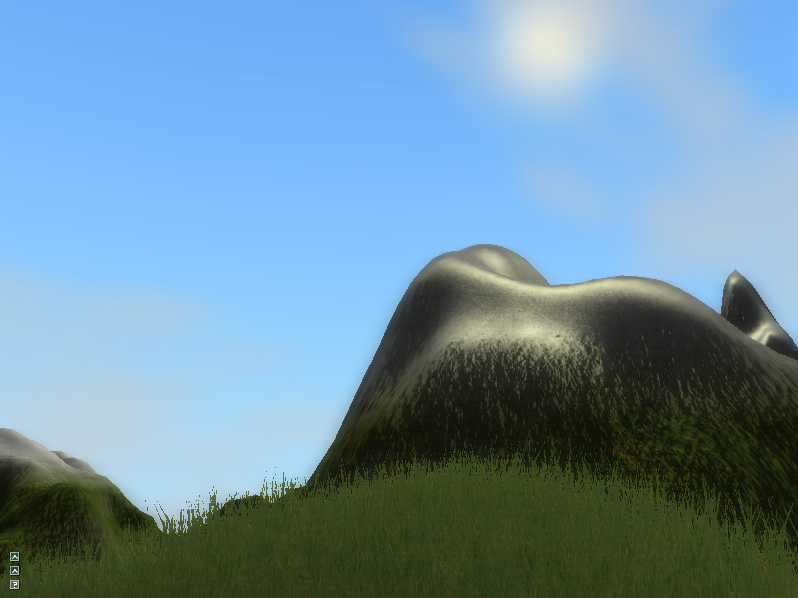
\includegraphics[width=12cm]{frontpage}
    \vspace*{40pt}
    \\
    \begin{minipage}{0.4\textwidth}
      \centering
      Asger Dam Hoedt \\ asgerhoedt@gmail.com \\ 20051770
    \end{minipage}
    \begin{minipage}{0.4\textwidth}
      \centering
      Christian P. V. Christoffersen \\ cpvc@cs.au.dk \\ 20050879
    \end{minipage}
}
\vfill
\small
Department of computer science\\
Aarhus Universitet
\end{titlepage}

\clearpage\pagenumbering{Roman}
\tableofcontents

\clearpage\pagenumbering{arabic}


%\maketitle

% -*- mode: latex; mode: auto-fill; coding: utf-8; -*-

\chapter{Introduction}
This report is the product of the second part of the course:
Introduction to Computer Graphics, followed by the authors during the
spring of 2010 at the department of computer science at Aarhus
University. The focus of this second part of the course is OpenGL's
programmable pipeline and OpenGL extensions.

To utilize the power of these advanced rendering technologies we have
chosen to try and make a realistic looking outdoor environment. The
project is based on a previous OpenEngine project, but most of it has
been rewritten as part of this project.

\section{Setting the scene}
When creating a scene in computer graphics the director, as when
making a movie or directing a play, writes a script. This script
includes descriptions of the mood and the setting where the story
unfolds.
%
This report describes techniques for rendering a scenery 
where the authors had the following setting in mind.
%
The scene consists of an island surrounded by a calm ocean as far
as the eye can tell. The island has sandy beaches, fields of grass
waving gently in the breeze, and tall mountains with pure white snow
on the top. Clouds are drifting on the breeze and in the horizon
the sun is setting, casting it's last golden rays toward the
landscape.

\section{Previous work}
This project is build ontop of a previous heightmap project in the
OpenEngine framework. While that old project's only purpose was to
explorer heightmap techniques, this project has been about making the
environment more aesthetically pleasing. Alot of effort have therefore
gone into the shaders, both with respect to creating a more realistic
result and optimizing them, this means that none of the old shader code
remains. Most of the code behind the heightmap scene node have also
been completely rewritten to better facilitate extensions made in this
project and for future extensions.

The water used in this project was made by the authors as part of
the old heightmap extension, but contains most of it's original code,
appart from using the new \class{FrameBuffer} abstraction.

Apart from the terrain, we have extended the scene with an
animated skydome, waving grass and post process effects.

%% We have previously been work on this project, but not been satisfied
%% with the mood of the result because only the basic objects in the
%% scene was put into play. In this project we want to focus our
%% attention on the making the details of an outdoor scene seem realistic
%% and convincing. In our previous work the island was implemented as a
%% height map, where the ocean was plane separating the terrain into an
%% underwater environment and land environment. The differentiation of
%% sandy beach, grass fields, rocks, and snow was based on height and
%% rendered by interpolating different textures for each type.

%% \section{Rendering outdoor scenes}
%% To create a more convincing and realistic outdoor scenery we need to
%% add more details than done in our previous work. This includes
%% improving the details of the landscape by using more advanced
%% lighting, animated grass that waves in the wind, a realistic looking
%% sky, and added post processing effects.

\section{OpenEngine}
The work presented in this report is build on top of the OpenEngine
framework. This framework is an open source project that was started
at Aarhus University in the spring of 2007, and was original build to
teach the course Computer Game Development, CGD, the same year. The
authors of this report are both deeply involved in the ongoing
development of OpenEngine, and have been so since its beginning.

OpenEngine is a framework for rendering 3D scenes using a scene graph.
For our project we have mostly implemented new scene graph nodes, such
as \class{HeightmapNode}, \class{MeshNode} or \class{PostProcessNode},
where the two latter were developed during the process of creating
this project and have made their way into the core framework. We use
the two existing nodes; \class{TransformationNode}, for translating
the skydome, and \class{BlendNode}, to make the skydome transparent.\\

OpenEngine is composed of a core framework, extensions, and
projects. In this project we have made use of some already available
extensions:

\begin{itemize}
  \item \code{SDL}, to create a window and get an OpenGL context.
  \item \code{GenericHandlers} for keyboard and mouse event handling.
  \item \code{CairoResource} and \code{HUD} to draw and render the FPS
    counter ontop of the rendered image.
  \item \code{AntTweakBar}, \code{Inspection}, and
    \code{InspectionBar} to add graphical components, allowing us to
    change values of variables at runtime.
\end{itemize}

The following extensions are also used in our project and have either
been created or extended during the implementation of our project:

\begin{itemize}
  \item \code{OpenGLRenderer} which handles all interaction with
    OpenGL inside the OpenEngine framework. This includes the
    allocation of \emph{textures}, \emph{vertex buffer object} and
    \emph{frame buffer objects} on the graphics card and a
    \class{RenderingView} that traverses the scene graph and renders
    it. During this course the OpenEngine core and this extension have
    been extended with buffer object support, three dimensional
    textures, new GLSL shader implementation and our
    \code{PostProcessNode}.
  \item \code{FreeImage} was wrapped in an extension and enables us to
    load and save \code{PNG}, \code{TGA} and \code{EXR} images,
  \item \code{MeshUtils} which was created as part of the new geometry
    structure to handle  buffer objects. It creates the geodesic
    spheres used for the skydomes.
  \item \code{TexUtils} which includes our noise generation algorithm
    described in chapter \ref{chap:noise},
  \item \code{OpenGLPostProcessingEffects} which holds shaders for
    some of the effects described in chapter \ref{chap:pp} and a lot
    of other effects.
  \item \code{Heightmap} which implements a heightmap node and a grass
    node. This extension also includes an expansion to the
    renderingview in \code{OpenGLRenderer}, which can render the
    heightmap and grass.
\end{itemize}

All of these extensions are used by our \code{Terrain} project, which
sets up the scene and holds modules for handling logic, like passing time of
day or sun direction to shaders.

% Which extensions contain the important code parts, and include
% filenames in appendix

To utilise OpenGL's programmable pipeline we chose to use the OpenGL
Shader Language, GLSL, instead of NVIDIA's CG. This was partly due to
our previous experience with GLSL and partly because a lot of work had
gone into optimizing and extending the OpenEngine GLSL shader
implementation in the first quarter of the course.

\section{OpenGL version and extensions}
% Antager opengl 2.1 som core så brugte extensions

Since every new version of OpenGL is composed of a set of extension,
OpenGL now consists of quite a large number of these
extensions. Therefore instead of listing every extension used in this
project, OpenGL 2.1 is assumed and only extensions not in this version
will be listed. The extensions used in our project are described in
appendix \ref{sec:GLext}

%%% Local Variables:
%%% mode: latex
%%% TeX-master: t
%%% TeX-PDF-mode: t
%%% End:


\chapter{Heightmap}

% A few lines about heightmaps

The terrain itself in our demo is generated from a heightmap and is a
continuating on the work that we did in the first quarter (which
itself was based on earlier work). How a heightmap is loaded from a
texture and converted to geometry is pretty straight forward, and thus
won't be our focus here. Instead we will focus on our lighting model
and how it was derived from the generel lightmodel presented in
Real-time Rendering. We will talk about how we give the illusion of
more detailed geometry by implementing bump maps, which requires us
move the bumped normal in tangent space. Finally we will explain how
texture arrays where used to cut back on texture unit usage and
texture lookups when rendering.\\

% Geomorphing because it is in the vertex shader
However before we start on all the cool visuel effect, we must briefly
touch upon the subject of geomorphing to understand part of what is
going on in the vertex shader.\\



\section{Lighting}

Because we're using shaders for rendering the heightmap, we need to
implement our own lighting effects. Since we're outside and rendering
natural environment our only lightsource is the sun, which is a
directional light. This allows us to ignore several aspects of the
lighting equation for one light source, equation 4.19 in Real-time
Rendering. 

\begin{displaymath}
  \mathbf{i}_{tot} = \mathbf{a}_{glob} \otimes \mathbf{m}_{amb} +
  \mathbf{m}_{emi} + c_{spot}(\mathbf{i}_{amb} + d(\mathbf{i}_{diff} + \mathbf{i}_{spec}))
\end{displaymath}

First of since we only have one lightsource in our entire
scene, the global ambience can be taken into account in the
lightsource's ambience, removing that expression from the
equation.

\begin{displaymath}
  \mathbf{i}_{tot} = \mathbf{m}_{emi} + c_{spot}(\mathbf{i}_{amb} + d(\mathbf{i}_{diff} + \mathbf{i}_{spec}))
\end{displaymath}

Also our lightsource is a directional light, so the spotlight factor,
$c_{spot}$, and attenuation, $d$, can safely be removed.

\begin{displaymath}
  \mathbf{i}_{tot} = \mathbf{m}_{emi} + \mathbf{i}_{amb} + \mathbf{i}_{diff} + \mathbf{i}_{spec}
\end{displaymath}

Lastly our emission factor is 0, so we end up with

\begin{displaymath}
  \begin{array}{rl}
    \mathbf{i}_{tot} &= \mathbf{i}_{amb} + \mathbf{i}_{diff} +
    \mathbf{i}_{spec}\\
    &= \mathbf{m}_{amb} \otimes \mathbf{s}_{amb} + (\mathbf{n} \cdot
    \mathbf{l}) \mathbf{m}_{diff} \otimes \mathbf{s}_{diff} +
    (\mathbf{v} \cdot \mathbf{r})^{m_{shi}} \mathbf{m}_{spec} \otimes
    \mathbf{s}_{spec} 
  \end{array}
\end{displaymath}

where we have used the following three formulas for ambient, diffuse
and specular lighting.

\begin{displaymath}
  \mathbf{i}_{amb} = \mathbf{m}_{amb} \otimes \mathbf{s}_{amb} 
\end{displaymath}

\begin{displaymath}
  \mathbf{i}_{diff} = (\mathbf{n} \cdot \mathbf{l}) \mathbf{m}_{diff} \otimes \mathbf{s}_{diff} 
\end{displaymath}

\begin{displaymath}
  \mathbf{i}_{spec} = (\mathbf{v} \cdot \mathbf{r})^{m_{shi}} \mathbf{m}_{spec} \otimes \mathbf{s}_{spec} 
\end{displaymath}

where $\mathbf{n}$ is the surface normal, $\mathbf{l}$ is the
direction of the light, $\mathbf{v}$ is the vector pointing from the
camera to the surface point and $\mathbf{r}$ is the reflection of the
light around the normal. All the vectors are assummed to be normalized
and can be seen on figure ??

% @TODO add vector figure

% @TODO add images
The contribution of each factor to the final image can be seen in figure ??

Now if we restrict our material to only specify one color instead of a
seperat color for ambient, diffuse and specular, we can reduce the
equation to 

\begin{displaymath}
  \begin{array}{rl}
    \mathbf{i}_{tot} &= \mathbf{m}_{color} \otimes \mathbf{s}_{amb} + (\mathbf{n} \cdot
    \mathbf{l}) \mathbf{m}_{color} \otimes \mathbf{s}_{diff} +
    (\mathbf{v} \cdot \mathbf{r})^{m_{shi}} \mathbf{m}_{color} \otimes
    \mathbf{s}_{spec} \\
    &= \mathbf{m}_{color} \otimes (\mathbf{s}_{amb} + (\mathbf{n} \cdot
    \mathbf{l}) \mathbf{s}_{diff} + (\mathbf{v} \cdot
    \mathbf{r})^{m_{shi}} \mathbf{s}_{spec}) \\
  \end{array}
\end{displaymath}

This restriction is more physically correct, in the sense that only
the color of the material is now shaded with respect to the different
light components, but is also more restrictive to artists.\\

In the above formulas the specular lighting has been given by the
Phong lighting equation, $\mathbf{i}_{spec} = (\mathbf{v} \cdot
\mathbf{r})^{m_{shi}} \mathbf{m}_{spec} \otimes \mathbf{s}_{spec}$,
where $\mathbf{m}_{spec} = \mathbf{m}_{color}$ and $\mathbf{r} = 2
(\mathbf{n} \cdot \ \mathbf{l}) - \mathbf{l}$.

A faster approximation was proposed by Blinn, where


\section{Bump mapping}



\section{Ground layers}



\section{Vertex shader}

% Geomorphing, fordele/ulemper, alternativer

% Terrain skal placeres i worldspace, acceptabel antagelse og spare os
% for matrix multiplicationer.

\section{Fragment shader}

% Light calculations (blinn/phong)

% Calculating the appropriate texture index and blending with the next
% layer.

% Normals and tangent space

% Bump mapping (rotating the normal in tangent space)

% Optimized texture lookup (saving 2 normals in 4 channels and
% blending them, not implemented)

\section{Summary}




% Place future work here or after the conclusion?

% Clip mapping, will make it easy to use LOD shaders (out with bump
% and specular) Also simply geometry LOD using alpha blending (take
% care to render geometry in the correct order)


%%% Local Variables:
%%% mode: latex
%%% TeX-master: t
%%% TeX-PDF-mode: t
%%% End:


\chapter{Waving Grass}

% GPU gems 1 chapter 7

A completely static terrain would appear quite lifeless. Some foliage
gently swaying in the wind would make the landscape seem more idyllic
and grass was therefore added.

Some considered rendering techniques for grass were

\begin{itemize}
\item Rendering grass straw textures on quads. This allows us to
  render several grass straws while only having to process 4
  vertices. Letting it wave in the wind is also easy as that only
  means moving the 2 top vertices. A problem however is that the
  illusion breaks down when viewed from above or on steep cliffs.
\item Modeling each grass straw. This technigue allows for very
  flexible grass with correct lighting. It is however very expensive
  to process all the vertices, so it's ususally used in conjunction
  with the above method for far away grass.
\item Rendering a volume texture containing the grass straws.
\end{itemize}

We opted for grass drawn onto quads, since it's easy to draw a quad of
grass on the screen and grass textures are easy to come by.

However the entire landscape can't simply be covered with millions of
quads of grass, as that would be extremely expensive to render, so
there are some design decisions to be made. Another problem with this
technique is that part of the grass texture is transparent, and
transparency isn't easy in the OpenGL 2.1 pipeline. A solution would
be depth peeling or z-sorting the straws, but for our purpose we
propose a much simpler method in the
\hyperref[sec:transparency]{Handling Transparency subsection}.

% @TODO reference GPU Gems 1

The basis of the grass implementation is Chapter 7 in GPU Gems 1. Here
they propose to draw the quads in objects with star patterns, to
achieve a grass effect independent of the cameras line of sight. Our
implementation does the same, but allows the user to specify how many
quads should be used used pr. star object. Setting this to 1
effectively disables the star pattern and simply renders random quads
of grass straws instead.

\section{Placing the grass}

As stated earlier we cannot simply draw the grass everywhere without
incurring a huge fps penalty, so instead we focus on drawing the grass
around the camera. We choose to draw it in a square around the camera,
but other shapes should be possible.

% explain algorithm

On \reffig{fig:grassTranslation} the basics of the algorithm can be
seen. We need to translate the square of grass centered around origo
to the camera. But we can't simply use the vector from origo to the
camera, since that would make the grass straws float along with the
camera. Instead we need grass straws exiting the square on one side to
overlap and appear on the other side. This can be achieved by ensuring
that grass objects are always moved by a multiplum of the grass
squares side's length, and is expressed in the following equation

\begin{displaymath}
    -halfSize \le position + size * n - eye \le halfSize, n \in N \\
\end{displaymath}

Focussing on the left hand side of the equation and remembering that
$n$ should be an integer, $n$ can be calculated as 

\begin{displaymath}
  \begin{array}{l}
    -halfSize \le position + size * n - eye \\
    \Updownarrow \\
    (eye - halfSize - position) / size \le n \\
    \Updownarrow \\
    n = \lceil (eye - halfSize - position) / size \rceil \\
    \Updownarrow \\
    n = \lceil (eye - position) / size - 0.5 \rceil \\
  \end{array}
\end{displaymath}

Now the new position of the grass straw is simply calculated by 

\begin{displaymath}
  newPos = position + size * n
\end{displaymath}

% And placing it in front of the camera


The grass quads have now succesfully ben placed in a square around the
camera, as can be seen on \reffig{fig:grassTranslation}. However most
of the straws still aren't inside the frustum. A small trick can be
applied to move more of the grass up in front of the camera. Instead
of placing the grass around the camera, it can be placed at a position
in front of it, relative to the cameras current direction. Since at
least half the grass square will be behind the camera, we choose to
move the camera position by the halfsize multiplied by the normalized
camera direction. This places the center of the grass in front of the
camera, but the border will never be in front of the camera. The
result is many more grass straws on the screen at the same vertex
processing cost.

% creation and one draw call

Since grass placed anywhere will now be translated to the camera, we
can create it anywhere we like. More importantly all the quads of
grass straws can now be drawn with one single draw call, and the
vertex shader will translate it to the camera. This removes a major
overhead we could have had if all quads should have been drawn
individually.

% Placing it on the heightmap and normal lookup

Our next hurdle is placing the grass straws on the terrain. Since
we're continuesly translating the grass quads, we can't know their
correct height at creation time and must therefore calculate it in the
vertex shader. We therefore calculate a texture coordinate from the
grass position and use that to lookup into the heightmap texture,
where we can find the correct height for the grass. To ensure that the
terrain and grass are equally lighted (lit?), we use the same
procedure to lookup into the heightmaps normalmap.

% not on sand or snow.

The last part of the grass placement is to keep it off the sand, snow
and steep cliffs. To this end we pass along the center of the grass
straw to the vertex shader. The center is then subjected to the same
translations as the vertex position. Wether or not the grass straws
should be visible can then be estimated from the height of the
center. If the center is too low the grass is on sand and should not
be visible, likewise if the center is too high it is snow. A similar
scheme is used for deciding if the grass is above cliff, where the
height is replaced by the normal.

The reason for using the center of the grass objects is that while one
side of the quad may be placed perfectly legal, the other side could
be placed on sand or snow. In order to collapse the grass objects we
needed a constant variable across the objects and that was the center.


\section{Waving in the wind}

Our animation algorithm is the same as the one proposed in section
7.4.4 of GPU Gems 1, where the grass objects center is used to create
'local chaos'. This means that all the grass can still be drawn with
only one draw call, texture are minimally distorted since the vertices
always have the same distance to their neighbours and the local chaos
creates a more natural wave effect. Of the two cons to the approach
only one of them applies to our implementation. The first con, which
is that extra uniform data is required to hold the center of the grass
object, doesn't apply ion this case, since the center was needed
anyway. The second con does apply to our shader, namely that the
complexity of the animation algorithm is limited in order to minimize
the cost of the shader. The wave therefore is just a simple cosine
function applied to the two top vertices, distinguished by their
texture coordinate.


\section{Handling Transparency}\label{sec:transparency}

% Discarding seethrough texture (how to avoid z sorting and rendering
% everything with one draw call)

With the grass placed on the terrain, texture transparency needs to be
handled. The grass straw texture can be seen in
\reffig{fig:grassStraws}. Since everything is drawn with one draw
call, z-sorting every frame isn't an option. Instead the transparency
and drawing order issue is completely ignored, by only rendering
completely opaque fragments or discarding them. This is done in the
fragment shader, where colors with alpha values below a certain value
are simply discarded. The reason for not just discarding everything
stictly below 1 is that mipmapping has to be taken into account. If 2
opague and 2 transparent pixels are combined in a lower mipmap layer,
that would yield an alpha of 0.5, but the fragment should perhaps
still be rendered. In practice we found that discarding alphas below
0.6 works well with the grass straw texture.

\begin{figure}
  \label{fig:grassStraws}
  \centering
  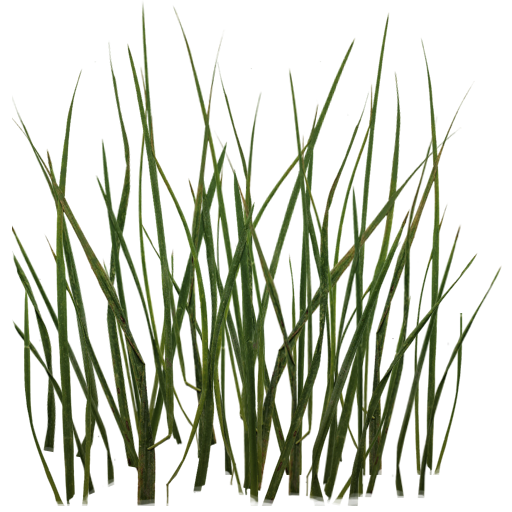
\includegraphics[width=5cm]{grassStraw}
  \caption{The grass straws.}
\end{figure}

% Simple diffuse lighting, no specular.

%%% Local Variables:
%%% mode: latex
%%% TeX-master: t
%%% TeX-PDF-mode: t
%%% End:


% -*- mode: latex; mode: auto-fill; coding: utf-8; -*-

\chapter{Sky}
An essential part of an outdoor environment is the sky, whether it is
night, day, cloudy or clear sky plays an important roll in setting the
mood of the scene. The sky is an ever changing part of any outdoor scene
and depends on many things including both the time of the day and on the
weather conditions.
%
This makes it a hard effect to simulate and visualize, but because it
is such a central part of an outdoor setting, it must be included in
the rendering.

Historically, skies in computer graphics, like many other visual
effects, started of as a simple thing. For a long time, the sky way
simulated by a simple light blue background color, which works fine
when used together with simple scene. But as the other objects in the
scene has become more complex and detailed this simple approach makes the
sky stand out. Therefore developers have started to use sky boxes,
which is a technique that maps images of the sky onto a box. This box
then surrounds the entire scene and the camera is inside the box at
all times, making the illusion of fare stretching planes by using
simple images.
%
One problem with using a box when doing this, is that the edges between the
images on different sides of the box are apparent as artifacts when
looking directly at them. To get around this problem, developers
instead use a sphere or dome as the basic geometry, and hence the name
sky dome, when rendering the sky. The main difference between these
two approaches is the texture mapping of the images. When mapping
images onto a box a straight forward approach can be used, but when
using a dome this step becomes much more tricky.

Returning to the images used when mapping a sky box or dome. When
using stills the sky seams static and dull. By animating ...

\section{Sky domes}
We have chosen to using two sky spheres, one inner sphere for
rendering white clouds with alpha transparency, and an out sphere to
render a background color which can change based on the time of day.
We also include cloud animation based on a simple model for wind, so
the clouds change over time.

\subsection{Geometry}
We have tried two different ways on generating the sphere
geometry. The first method used was the traditional longitudinal/latitude
sphere commonly used for geographical maps. This
however gave very obvious image stretching artifact at the poles
because of oversampling in these regions. Instead we now use geodesic
spheres which consist of equilateral triangles and are beautifully
constructed by recursively subdivision of an icosahedron until the
required LOD is attained.

\subsection{Atmospheric dome}
What phenomena drives the coloring of the sky, making it so beautiful
with it shades of blue and red?
This is the questing ask by researchers studying 
\emph{atmospheric scattering}. This subject has been studied in great detail,
an lots of complex theories and models has been developed within the
field.
We however have chosen not dig deep into this subject because it could
be an entire subject of its own.

However, to color our sky we use a simple model based on color
gradients as described in ref:\footnote{A fast, simple method to
  render sky color using gradients maps, by Jesús Alonso Abad.}
Where the atmospheric dome is colored based on time, height, and the
location of the sun.
We use a color gradient e.g from light to medium blue as a function of
the height and dividing the time into four periods: day, night,
sunrise and sunset, and use the location of the sun the make a
beautiful sunrise and sunset.

\subsection{Cloud Dome}

\subsubsection{Cloud texture}
We have chosen to use a procedural generated image to visualize the
clouds. By take this approach we can change their appearance and
generate very different looking clouds by only altering a few
parameters that is supplied to the generation algorithm.

We have furthermore chosen a three dimensional image because this
eases texture mapping when the image is to be mapped onto the sphere.

\subsubsection{Procedural generated images}
To generate the cloud image we have been inspired by an Internet
homepage\footnote{\url{http://freespace.virgin.net/hugo.elias/models/m_clouds.htm}
  \\(Be want though, this homepage does not use Perlin noise as they
  say but value lattice noise)}
describing how to use procedural generation and
image layering/composition in combination to produce texture that
looks like real clouds.

Procedural generation, is a very fuzzy term, which covers quite a
large area.
--> ref. PG 3rd edition

But boils down to, using some kind of algorithm to produce data, where
a number of parameters can be specified to control the
generation process in a way that alters the result in a intuitive way
based on the parameters.

The basic building block when generating procedural data are noise
functions. A noise function is a function e.g. $f(x)$ which for 
---> ref. PG3rd edition

There are many noise functions, with different properties. But general
they are divide into categories based on how they generation the
noise.

Value lattice noise.

Gradient noise which is the category the includes the most 
now famous noise function known as Perlin noise, first described by Ken
Perlin in famous 1985 paper: Making Noise. 


\subsubsection{Texture mapping - animation}
The basic texture mapping scheme, is to put the three dimensional
texture into a unit cube, and use texture coordinates based on the
unit sphere to make a direct mapping which avoids texture stretching.

If we only did this, the a large portion of the generated texture
would not be used.

So besides the basic texture mapping scheme, we have introduced
texture coordinate animation. This has been done by modeling the wind.







%%% Local Variables:
%%% mode: latex
%%% TeX-master: t
%%% TeX-PDF-mode: t
%%% End:



% -*- mode: latex; mode: auto-fill; coding: utf-8; -*-

\chapter{Procedural generation of content}
\label{chap:noise}
What is known as procedural or synthetic generation of content are
used extensively in computer graphics to enable generation of natural
looking details. By generating details, in contract to doing them by
hand, boring work typically done by computer artists can be cut down,
and instead be used on designing the overall look and feel.
%
The term procedural generation of content is very fuzzy and covers
quite a large area of different techniques, but boils down to some
kind of algorithm that produces data \citebook{page~12}{ebert2003}.
Typically where a number of parameters can be specified to control the
generation process in a way that alters the result in a intuitive way
based on the parameters.

\section{Generating irregular data}
We have chosen to concentration our effort on irregular data generation
minded on textures, therefore only this type type of data generation
will be covered in the following.
%
The basic building blocks when generating irregular data are
noise functions. A noise function is a function that is apparently
stochastic and will break up monotony of the patterns that would
otherwise be too regular \citebook{page~67-78}{ebert2003}.
%
Typically a noise function is a function of the space so the arguments
can be filled directly when rendering, e.g. $f(x,y,z)$.
%
An obvious stochastic primitive is uniformly distributed random
numbers with no correlation, which is also known as white noise.
In computer graphics however true random numbers are rarely used,
because they are not controllable.
Instead pseudo random number (PRN) generators are used to produce a
fair approximation to white noise. These however are controllable and
furthermore produce the same number sequences on two successive runs
provided the algorithm is started with the same preconditions.
%
Another property of white noise that we do not want is that it is
uncorrelated in all function values. This causes problems in computer
graphics because of rounding errors in the floating point
representation used when rendering. Instead we use a low-pass filtered
version of an approximation to white noise.

There are many different ways of using PRN to produce noise functions,
each method generate functions with different properties. General the
functions are divide into categories based on how they generate the
noise. To making an important and often misunderstood point regarding
what precisely defines the famous Perlin noise function, we will
introduce two basic categories of noise functions: Value and gradient
noise, which both also are categorized as lattice noise.

%\pagebreak

\subsection{Lattice noise}
In geometry a lattice is a discrete subgroup (a set of points) in the
same dimension as the basis vectors spanning the vector space. A
lattice can be viewed as a regular tiling of space by primitive cells
forming a grid structure. The most used lattice in computer graphics is the
regular Cartesian grid, which can be viewed as a tiling of
squares in two dimensions, see figure \ref{fig:square-lattice}. For
clarity figure \ref{fig:lattices} also provides other examples of
lattices.

\begin{figure}[!h]
  \centering
  \subfloat[Triangle lattice.]{
    
\includegraphics[width=3cm]{200px-Equilateral_Triangle_Lattice}
    \label{fig:lattice1}
  }
  \hspace{4mm}
  \subfloat[Rhombic lattice.]{
    
\includegraphics[width=3cm]{200px-Rhombic_Lattice}
    \label{fig:lattice2}
  }
  \hspace{4mm}
  \subfloat[Square lattice.]{
    
\includegraphics[width=3cm]{200px-SquareLattice}
    \label{fig:square-lattice}
  }
  \hspace{4mm}
  \subfloat[Parallelogram lattice.]{
    
\includegraphics[width=3cm]{200px-Oblique_Lattice}
    \label{fig:lattice4}
  }
  \caption{Four simple lattice types in two dimensions.}
  \label{fig:lattices}
\end{figure}

Lattice noise is generated by having a lattice, and then for each
lattice point generating one or more random values for that point
depending on the type of noise we want.
%
The low-pass filtering is then done by interpolating the values at the
grid points to fill the entire space between the lattice
points. Different interpolation scheme can be used to calculate these
values, which yield different properties for the noise function.

\subsubsection{Value noise}
Value noise is the simplest type of lattice noise, here the values
stored at each grid point are the values that are interpolated and
returned when the function is evaluated.

\subsubsection{Gradient noise}
Gradient noise however have generates a gradient at each point in the
lattice, which is a vector with the same dimension as the number of
dimensions wherein the function is defined. The gradients in each grid
point is then used to calculate a continuous function between the grid
points, which again can be used to evaluate a noise value.
%
The gradient noise category includes the now famous noise
function known as Perlin noise, first described by Ken Perlin in
his famous paper: \citeabook{Perlin85}.
%
Here it is time once again to warn the reader that many authors of web
pages,
e.g. \url{http://freespace.virgin.net/hugo.elias/models/m_perlin.htm},
seems to confuse Perlin noise with value noise, with the result that
an Internet search for Perlin noise becomes a non-trivial job.

\section{Composite of layers}
Noise alone does not make realistic looking textures, only by carefully
choosing the noise parameters and cleverly combining many layers of
different looking noise results in naturally beauty. In the following,
we will focus on generating a volumetric texture of clouds, but the
description illustrates the overall process of how to generate and
combine noise functions.
%
To enable writing of how to combine noise functions, we will borrow
terminology from the field of digital signal processing (DSP).
In DSP the term \emph{sample frequency}
describes the space between to consecutive samples, and the term
\emph{amplitude} the maximum value of the function.

To generate the basic shape of some clouds we use a low
frequency noise with a large amplitude as illustrated for an one
dimensional case in figure in \ref{fig:1d-layer0}.
%
We add layers of details onto this low frequency noise by combining it 
with noise of higher frequencies.
%Where the details comes from the higher frequencies.
Because we want the basic shapes to be the most
dominant the amplitude of noise with higher frequencies are lowered,
this is shown in figure \ref{fig:1d-layer1} and \ref{fig:1d-layer2}.
%
We change these frequency and amplitude in octaves because
octaves frequent occur in nature and gives good visual results.
For each level of detail that is added the frequency is doubled while
the amplitude is halved. To illustrate this, we have used value noise
to generate three layers and combined them into the result show in
figure \ref{fig:1d-result}.

\begin{figure}[!h]
  \centering
  \subfloat[Layer 0.]{
    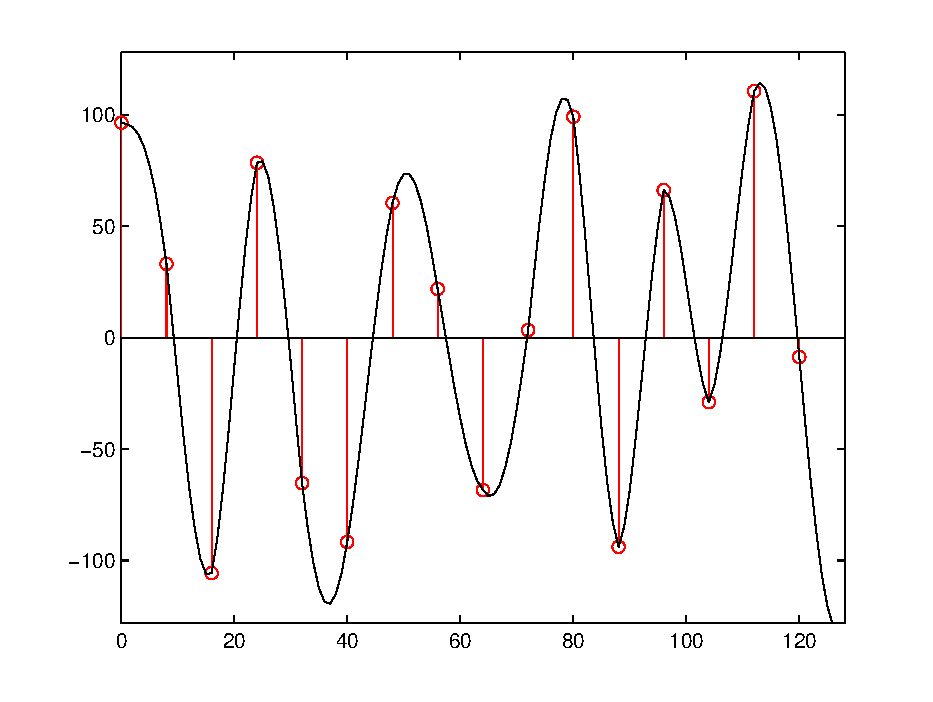
\includegraphics[width=7.25cm]{n0}
    \label{fig:1d-layer0}
  }
  \hspace{4mm}
  \subfloat[Layer 1.]{
    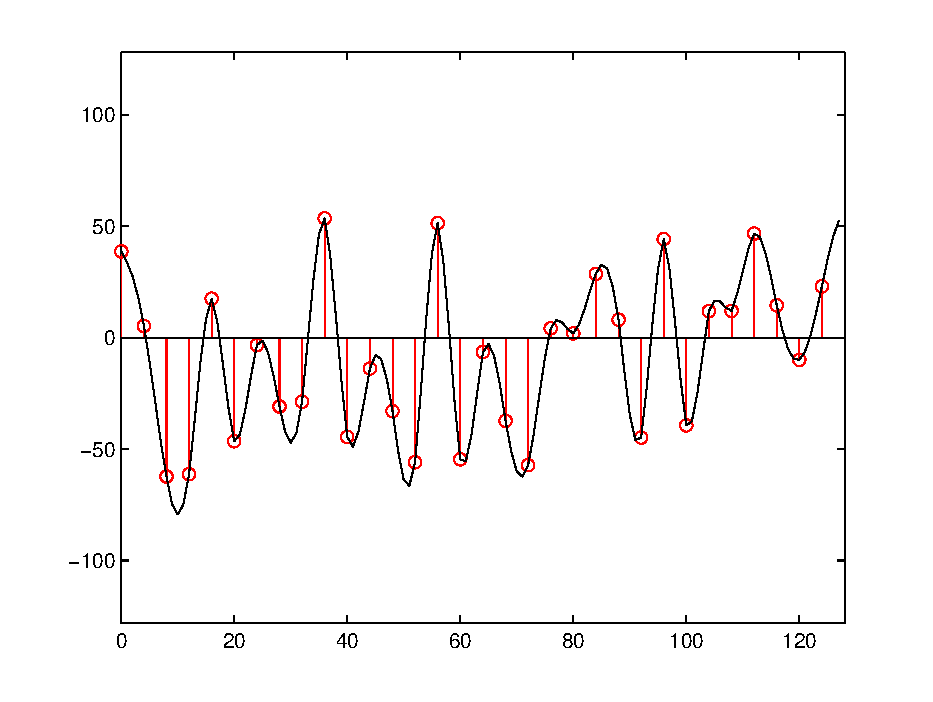
\includegraphics[width=7.25cm]{n1}
    \label{fig:1d-layer1}
  }
  \newline
  \centering
  \subfloat[Layer 2.]{
    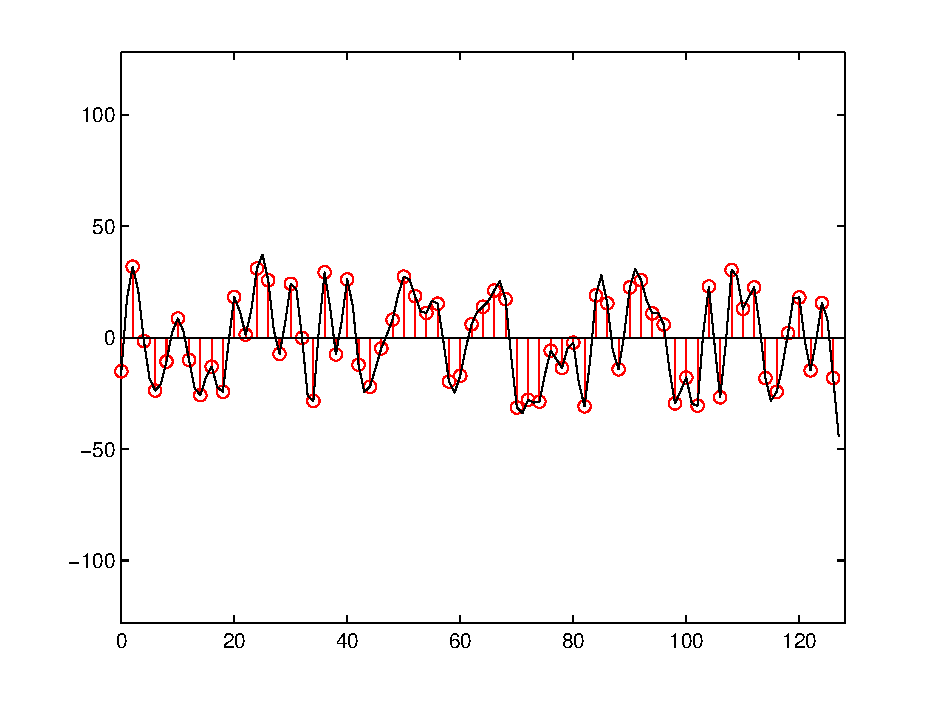
\includegraphics[width=7.25cm]{n2}
    \label{fig:1d-layer2}
  }
  \hspace{4mm}
  \subfloat[Result.]{
    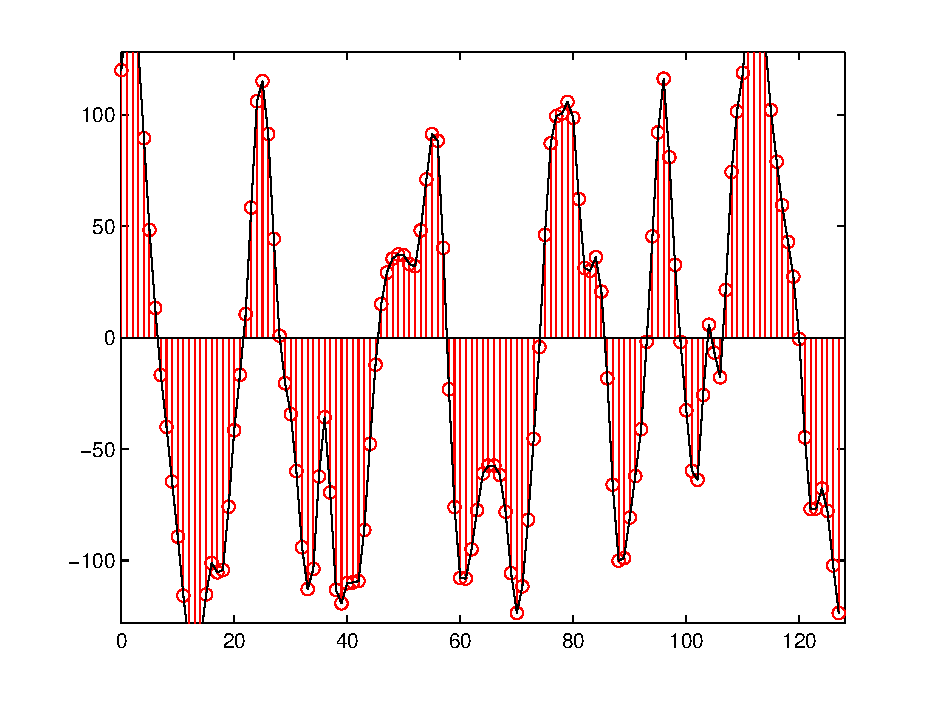
\includegraphics[width=7.25cm]{n0to2}
    \label{fig:1d-result}
  }
  \caption{One dimensional example of the combination process.}
  \label{fig:1d-layers}
\end{figure}

%\pagebreak
Moving into two and three dimensions are straight forward. Figure
\ref{fig:noise-layers} shows four layers of two dimensional white
noise rendered as alpha transparency on a fully white image, the blue
background has been inserted so the transparency can be seem. These
layers are the basic primitives for the upcoming combination into an
image that looks like clouds.
%
When sampling into an array, as has been done in figure
\ref{fig:noise-layers} the increase in sampling frequency is the same
as using a larger array. If this array represent an image or
texture, as in the figure, then the different layers do not have the
same height and width. To solve this, when algorithmically combining
two layers, the image with the lowest resolution is re-sampling to the
same resolution as the other image.

\begin{figure}[!h]
    \centering
    \subfloat[Layer 0.]{
      \colorbox{Cerulean} {
\includegraphics[width=3cm]{generated-rx8-b1024}}
      \label{fig:noise-layer0}
    }
  \hspace{4mm}
  \subfloat[Layer 1.]{
    \colorbox{Cerulean} {
\includegraphics[width=3cm]{generated-rx16-b512}}
    \label{fig:noise-layer1}
  }
  \hspace{4mm}
  \subfloat[Layer 2.]{
    \colorbox{Cerulean} {
\includegraphics[width=3cm]{generated-rx32-b256}}
    \label{fig:noise-layer2}
  }
  \hspace{4mm}
  \subfloat[Layer 3.]{
    \colorbox{Cerulean} {
\includegraphics[width=3cm]{generated-rx64-b128}}
    \label{fig:noise-layer3}
  }
  \caption{Four noise layers.}
  \label{fig:noise-layers}
\end{figure}

The layers are then combined two at the time. The process starts by
combining the two layers with lowest resolution. Then the result of
the previous combination is combined with the image with third lowest
resolution and so on.
%
Because we use linear interpolation between our lattice point, the
result of combining the layers, becomes very blocky looking, like the
image in figure \ref{fig:combined-layer1}. To get
around this we blur the result after each new layer is added, which
can be seem in figure \ref{fig:combined-layers}.

\begin{figure}[!h]
    \centering
    \subfloat[Combo of layer 0 to 1.]{
      \colorbox{Cerulean} {
\includegraphics[width=3cm]{combined-l1-b512}}
      \label{fig:combined-layer1}
    }
  \hspace{4mm}
  \subfloat[Combo of layer 0 to 2.]{
    \colorbox{Cerulean} {
\includegraphics[width=3cm]{combined-l2-b256}}
    \label{fig:combined-layer2}
  }
  \hspace{4mm}
  \subfloat[Combo of layer 0 to 3.]{
    \colorbox{Cerulean} {
\includegraphics[width=3cm]{combined-l3-b128}}
    \label{fig:combined-layer3}
  }
  \hspace{4mm}
  \subfloat[Result.]{
    \colorbox{Cerulean} {
\includegraphics[width=3cm]{output}}
    \label{fig:combined-result}
  }
  \caption{Snapshots of the combination process.}
  \label{fig:combined-layers}
\end{figure}

The final touch, after the image is generated, is to filter the image
with an exponential function which creates the look seen in figure
\ref{fig:combined-result}.

\section{Implementation}
When implementing noise functions, one must chose where the
computations are placed. One option is to do all computations as
pre-computations and then use the resulting noise texture for look up
at run-time. Another option is to do all the computations at
run-time. The main advantage of doing the calculation as pre-computation
is an increase in run-time performance, where as doing the calculations
at run-time enable adaption in LOD in relation to the camera
position. For the run-time computations to be fast enough for
real-time rendering they are usually done on the GPU, but although noise
functions exists in the GLSL API\citebook{}{}, they are not recommended because
their behavior are not specific by the specification and are
implemented differently in hardware by different vendors and on different
hardware generations. Developers that still want to do the calculations
at run-time, instead use a hybrid solution, generating a small noise
texture which can be used to implement more sophisticated noise
function on the GPU.
%
We however have chosen to do all the calculations as pre-computations
implemented on the CPU, our implementation is based the
\code{RandomGenerator} class of OpenEngine which again is based on the
PRN from \citebook{page~278-283}{NRIC2}.
%
The entire algorithm of generating noise, composing layers, and
blurring them is implemented as the following recursive function:

\begin{lstlisting}[frame=,language=C++]
    static FloatTexture2DPtr Generate(unsigned int xResolution, unsigned int yResolution,
                                      unsigned int bandwidth, float mResolution,
                                      float mBandwidth, unsigned int blur,
                                      unsigned int layers, RandomGenerator& r) {
            FloatTexture2DPtr noise =
                    CreateNoise(xResolution, yResolution, bandwidth, r.UniformInt(0,256));
            if (layers != 0) {
                FloatTexture2DPtr small = 
                    Generate(xResolution * mResolution, yResolution * mResolution, 
                             bandwidth * mBandwidth, mResolution, mBandwidth,
                             blur, layers-1, r);
                noise = Combine(noise, small);
                Blur(noise, blur);
            }
            return noise;
    }
\end{lstlisting}

*** correct above names, include class PelinNoise.

%%% Local Variables:
%%% mode: latex
%%% TeX-master: t
%%% TeX-PDF-mode: t
%%% End:


\chapter{Post Processing}

% Why post processing? Cool effects that can easily be applied to any
% project and reused.

In the previous sections we've had to use geometry to help us create
the landscape, sky and rendering it to the screen. Now we will turn to
screen space effects, which doesn't rely on geometry, but will instead
use the final color image and the depth buffer to create the
effects. Depth of field, motion blur and a screenwide glow are all
effects that can easily be produced through post processing and there
are many more.

% Easy to use important. Should handle most of the setup

We will try to create a general framework inside OpenEngine that can
handle most effects with the programmer having to do as little setup
as possible. It should also be possible to layer post processing
effects on top of each other, for example to combine a cel shader with
edge detection or optimizing blurring by using a technique called
separable convolution.

\section{Structure}

In this section we will first outline the new scene node called post
process node and how it will help the programmer setup post
processing. Then we will discuss the specifics of rendering the scene,
applying the post process effect to it and how we eventually chose to
structure the rendering.

\subsection*{Post Process Node}

The post process node will apply a fragment program to manipulate the
image rendered while visiting subnodes. Therefore it of course
contains an IShaderResourcePtr that points to the effect. It also
contains a pointer to an OpenEngine FrameBuffer, which the scene is
rendered to, and another FrameBuffer where the scene with the effect
is rendered into. Why the effect is not simply rendered directly to
the backbuffer (or previous frame buffer in case of chained effects)
is explained in the Rendering subsection. The postprocess node also
has a list of ITexture2DPtr's where the final image can be stored
after the effect has been applied, this is useful for some
implementations of motion blur, that relies on the previous image
being availible.

In order to allow users of the PostProcessNode to focus on writing
their effects, the node will handle most of the setup as long as a few
naming conventions are followed. If a uniform named \textit{depth} is
detected then the subscenes depth texture will be bound to this
uniform. Similarly if \textit{imageN}, where \textit{N} is any
integer, is seen, then the FrameBuffer's \textit{N}'th color
attachment will be bound to that uniform. The same goes for the final
image and the uniform name \textit{finalImageN}. The node can also
decide to improve performance by not copying the final image, if this
isn't needed. Of course the previous image doesn't make sense in the
very first rendering, so when initialized the node binds the
not-processed scene image as the final image, and then after the first
frame it switches to the final image. And finally, if needed the node
will pass the time to the shader.

All of this has allowed us to cut back on doing setup and spend our
time writing cool and fun effects.

\subsection*{Rendering}

% render to a framebuffer

The first thing that needs to be done before switching to the new
framebuffer is to save the old state. This means saving the name of
the old framebuffer and the dimensions of the viewport.

Once the state has been saved we set the viewport size to the one
specified in the nodes framebuffer and proceed to bind the framebuffer
and clear the color and depth. The subscene is then rendered to the
framebuffer.

% Apply the effect with depth testing set to always

When the scene has been rendered we bind the previous frame buffer and
set OpenGL's depth function to always let fragments pass. We can do
this since we're applying a post process to the entire image and it's
cheaper performance wise than clearing the depth buffer each pass. The
depth test couldn't simply be disabled as that would disable writes to
the depth buffer aswell, and we are interested in keeping the depth
values or maybe modifying them through a post process.

With the previous framebuffer bound, we apply the post process shader
and render a rectangle to the screen. The rectangle is simply drawn
from (-1,-1) to (1,1). If no matrices are applied to these vertices,
then the rectangle will cover the screen.

% Store the final image

If our post process effect relies on the final image from the last
rendering, then now is the time to save it. However first we have to
initialize the final framebuffer and attach the final color images to
the post process shader. Then we blit the image with it's effect into
the final image framebuffer, rescaling the image if the source and
destination rectangles are not of the same size.

% Allows multiple postprocess nodes

\section{Post Pocess Effect}

In this section we will take to a short look at some of the different
post process efects that we have created.

\subsection{Motion Blur}

While motion blurring may not be critical to outdoor environments,
many projects still benifit from it. Therefore one of the criteria
to the post process node was that it would allow an easy motion blur
implementation for existing and future open engine projects.

Motion blurring can be done in several ways. The simplest way
conceptually is to store the last $n$ images and then blend them
together. This creates a nice blurring effect across the last few
frames. The problem is that we then need to store the last few frames
in memory, giving us a memory overhead of 8-16 textures. Another
problem is that the blurring is framerate dependent, so low framerates
will make the blurring excessive, while high framerates will make it
non existent.

Another approach was proposed in GPU Gems 3, where the previous
ViewProjection matrix is used to calculate the previous position of a
fragment and then accumulate the colors between the current and
previous position. This approach however only creates blurring if the
camera is moved. A car that drives past the camera will crystal
clear. Another problem is that the shader becomes quite complex and
timeconsuming.

The algorithm that we settled on combines a low memory footprint with
a fast shader. We simply store the previous image, which contain all
the previous images blended together, and then blend them together
with the current image. That way the effect from old images will tend
toward 0 and the motion blurring will produce nice looking blurred
'tails' on moving objects.

% @TODO image to show the effect

% @TODO shader in appendix

\subsection{Glow}

When looking at natural outdoor environments in bright sunlight,
colors seem to blur or smeer together. We would like to reproduce this
effect using a fullscreen glow post process. Initally we created the
effect with just a single shader. This shader first did a box blur on
the surrounding fragments and then blended that result with the
original fragment. This produced the results we where after, but at a
huge performance overhead. The problem was texture lookups. To blur
the surrounding fragments of an $N \times N$ rectangle, we required
$N^2$ texture lookups. We solved this by applying the separable
convolution technique. In the first post process pass a horizontal
blurring is performed, then in the second pass a vertical blurring is
performed on the resulting image of the previous pass and this is then
blended together with the original non-blurred scene. For an $N \times
N$ rectangle we've now reduced $N^2$ texture lookups to $2N$, while
achieving the same effect.

% @TODO show the non blurred + blurred = glow images

As the images show, a subtle smeering gives a smoother and more
natural looking image.

% @TODO shader in appendix

\subsection{Depth of field}

When filming or photografing through a lens an effect called depth of
field occurs.

% @TODO shader in appendix

\subsection{Under Water}

% Combines the previous effects and a wobble

% Create it as several layered effects? Should be possible.

% @TODO shader in appendix

\subsection{Conclusion}

Storing and rebinding the previous framebuffer means that we can chain
several post process nodes together to form complex effects or
minimize the cost of applying an effect by using for example separable
convolution.

% One/two fbos pr node is a waste but makes it easy to setup and they
% can be configured individually

% Next step is merge



%%% Local Variables:
%%% mode: latex
%%% TeX-master: t
%%% TeX-PDF-mode: t
%%% End:


% -*- mode: latex; mode: auto-fill; coding: utf-8; -*-

\chapter{Conclussion}


%Post Process

%% Storing and rebinding the previous framebuffer means that we can chain
%% several post process nodes together to form complex effects or
%% minimize the cost of applying an effect by using for example separable
%% convolution.

% One/two fbos pr node is a waste but makes it easy to setup and they
% can be configured individually

% Other effects have been implemented, like wobble, edge detection,
% pixelate and an underwater that combines...



\section{Future work}

Future work on the terrain itself would include a clipmap
implementation and level of detail not only on teh textures and
geometry, but also within the shaders. An example would be removing
specular lighting and bumpmapping on distant terrain. An alternative
to the current geomeorphing LOD system is alpha blending, which would
make transistions between LODs easier, but ofcourse requires us to
handle transparency.



An extension to the atmospheric dome is to include the location or
angle of the sun to make a more beautiful sunrise and sunset.


The next step for the \class{PostProcessNode} is to allow it to be
placed anywhere inside the scene graph and then merge the post
processed image with the rest of the scene. Also optimized versions of
the most commen effects could be made to increase performance and in
the case of Depth of Field remove the flickering that comes from only
sampling one focuspoint.



\appendix
\input{Glext}

\bibliography{refs}

\end{document}

%%% Local Variables:
%%% mode: latex
%%% TeX-master: t
%%% TeX-PDF-mode: t
%%% End:
